\documentclass[11pt]{article}

\usepackage{float}
\usepackage{hyperref}
\usepackage{graphicx}
% formatting
\usepackage{fullpage}
\usepackage{verbatim}
\usepackage{moreverb}
\usepackage{minted}
\usepackage{parskip}
\let\verbatiminput=\verbatimtabinput
\def\verbatimtabsize{4\relax}

\begin{document}
\title{EE142 Lab 0.5 - VNA Calibration}

\author{Vighnesh Iyer \\
Department of Electrical Engineering and Computer Sciences\\
College of Engineering, University of California, Berkeley}
\date{}
\maketitle

\section{Testing Cable Phase Stability}

\subsection{Two-Port Technique}
We connect a SMA cable between port 1 and 2. 

Before connecting the cable, the SMA connector's pin depth and dielectric depth are both checked and are within spec. Also, the SMA connector was examined under a stereo microscope and it was cleaned with a cotton swab and alcohol to remove surface contaminants (specks of dirt and metal fragments).

\begin{figure}[H]
	\minipage{0.50\textwidth}
	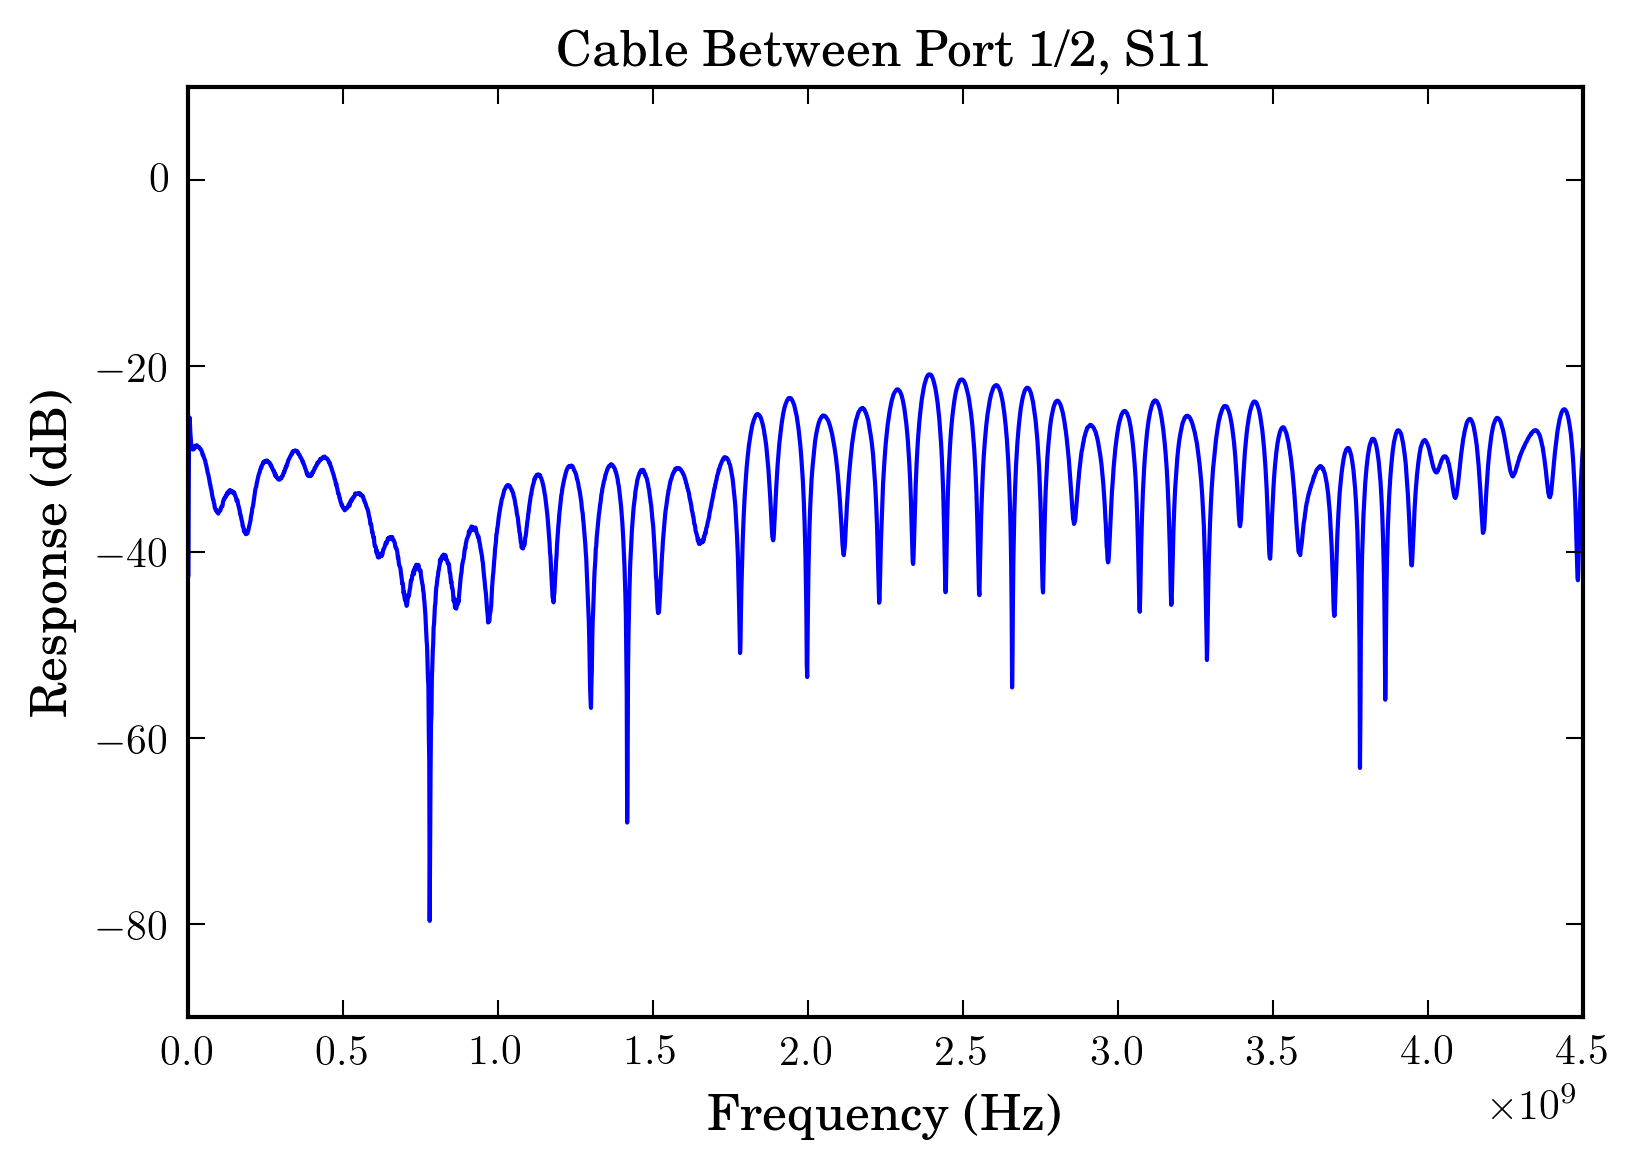
\includegraphics[width=\linewidth]{images/cable_phase_s11.png}
	\endminipage\hfill
	\minipage{0.50\textwidth}
	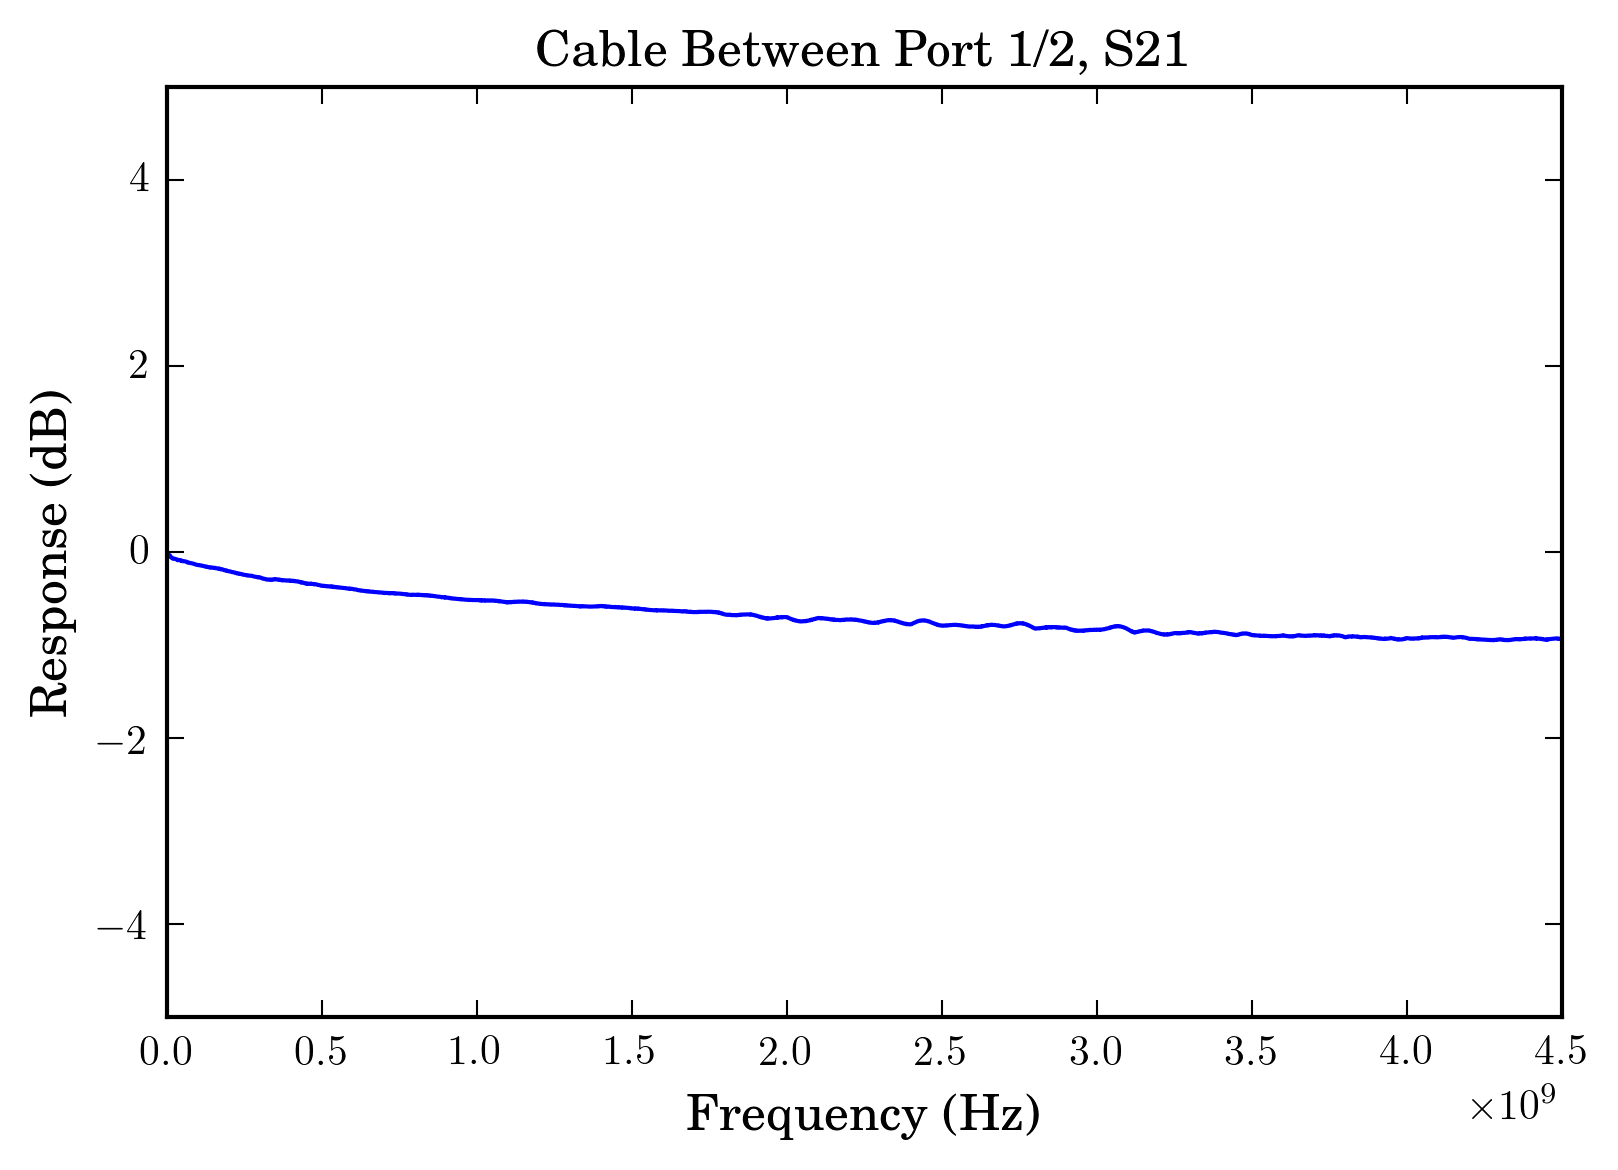
\includegraphics[width=\linewidth]{images/cable_phase_s21.png}
	\endminipage
\end{figure}

When plotting $S_{11}$, we see reflections and re-reflections 20 dB down which show discontinuities in the cable's impedance. When measuring $S_{21}$, we see that almost all the delivered power from port 1 makes its way to port 2 and we only see some drop-off at higher frequencies.

\subsection{One-Port with Cal Standard Technique}

We connect one end of a SMA cable to port 1 and the other end to a open calibration standard. The display is set to Log-Mag $S_{11}$.

The cable is placed down and we use the \verb|Data->Mem| = \verb|Data-Mem| to subtract out the last captured trace from the current trace. This pushes the Log-Mag trace to around -60 dB, but I expected the trace to plunge further down to -80 dB closer to the noise floor of the instrument.

Finally, the cable is moved around and flexed for 10 seconds, and the cable is placed down on the lab bench again. The trace is allowed to settle down.

The trace should have moved from its -80 dB state upwards as the cable's electrical length/phase has been slightly changed due to the movement. A very good cable moves to around -50 dB, while a decent cable moves to around -40 dB. A poor cable will move up to -30 dB or higher.

We can see that our chosen cable is of mid-range quality and has enough phase stability to perform reliable measurements.

\section{Calibration using E-Cal}

\section{Verifying Calibration With Cal Standards}
\end{document}
